\documentclass{article}

\usepackage{polski}
\usepackage[utf8]{inputenc}
\usepackage{graphicx}
\usepackage{float}
\usepackage{listings}
\usepackage{graphicx}
\usepackage{mathtools}
\renewcommand{\lstlistingname}{Funkcja}
\renewcommand{\theparagraph}{\alph{paragraph}) }\setcounter{secnumdepth}{4}
\lstset{language=C++,
numbers=left,
captionpos=b}

\author{Dominik Doberski, Artur Olejnik}
\title{
\huge Sprawozdanie 
\\Przetwarzanie równoległe\\
\Huge Projekt 2 PKG}

\begin{document}
\maketitle

\section{Wstęp}
\subsection{Temat}

Mnożenie macierzy - ukrycie kosztów transferu danych w czasie obliczeń (dla 5. wersji kodu), badania należy wykonać dla przetwarzania równoległego dla zbioru tablic jednocześnie dostarczanych, obliczanych i pobieranych do/z systemu PKG, porównanie z prędkością przetwarzania dla wersji 3.
\begin{itemize}
\item 5. wersja kodu -- grid wieloblokowy, obliczenia przy wykorzystaniu pamięci współdzielonej bloku wątków, zrównoleglenie obliczeń i transferu danych między pamięciami: operacyjną procesora, a globalną karty,
\item 3. wersja kodu -- grid wieloblokowy, obliczenia przy wykorzystaniu pamięci współdzielonej bloku wątków.
\end{itemize}
\subsection{Autorzy}
\begin{minipage}[t]{0.3\textwidth}
% Pierwsza kolumna (średnia)
Dominik Doberski\\
Artur Olejnik
\end{minipage}
\begin{minipage}[t]{0.15\textwidth}
% Druga kolumna (mniejsza)
132207\\
122402
\end{minipage}
\begin{minipage}[t]{0.55\textwidth}
% Trzecia kolumna (mniejsza)
dominik.doberski@student.put.poznan.pl\\
artur.olejnik@student.put.poznan.pl
\end{minipage}
\\\\\\
Grupa dziekańska I3\\
Termin zajęć: poniedziałek 16:50 
\subsection{Opis wykorzystywanej karty graficznej}
Do wykonania pomiarów wykorzystano program CodeXL. Testy zrealizowano na jednostce obliczeniowej o poniższej specyfikacji:
\begin{itemize}
\item Nazwa: Nvidia GeForce GTX 1060
\item Pamięć: 3072MB
\item Typ: dedykowana
\item CC – możliwości obliczeniowe: 6.1
\item Liczba SM: 9
\item Liczba rdzeni: 1152
\item Maksymalna liczba wątków na multiprocesor: 2048
\item Maksymalna liczba wątków na blok: 1024
\item Rozmiar osnowy: 32
\item Maksymalny rozmiar bloku: 1024x1024x64
\end{itemize}

\section{Analiza algorytmu}
\subsection{Kluczowe fragmenty kodu}
\subsubsection{Algorytm dla 3. wersji kodu}
Grid wieloblokowy, obliczenia przy wykorzystaniu pamięci współdzielonej bloku wątków:
\begin{lstlisting}[
caption={3. wersja kodu},
label=1. funkcja,
firstnumber=1]
template <int BLOCK_SIZE> __global__ void
matrixMul3(float *C, float *A, float *B, int wA, int wB ) {
    int bx = blockIdx.x;
    int by = blockIdx.y;
    
    int tx = threadIdx.x;
    int ty = threadIdx.y;
    
    int aBegin = wA * BLOCK_SIZE * by;
    int aEnd   = aBegin + wA - 1;
    int aStep  = BLOCK_SIZE;
    int bBegin = BLOCK_SIZE * bx;
    int bStep  = BLOCK_SIZE * wB;
    
    float Csub = 0;

    __shared__ float As[BLOCK_SIZE][BLOCK_SIZE];
    __shared__ float Bs[BLOCK_SIZE][BLOCK_SIZE];

    for (int a = aBegin, b = bBegin; 
    	 a <= aEnd;
    	 a += aStep, b += bStep) {
        As[ty][tx] = A[a + wA * ty + tx];
        Bs[ty][tx] = B[b + wB * ty + tx];
        
        __syncthreads();
        
#pragma unroll
        for (int k = 0; k < BLOCK_SIZE; ++k) {
            Csub += As[ty][k] * Bs[k][tx];
        }

        __syncthreads();
    }
    
    int c = wB * BLOCK_SIZE * by + BLOCK_SIZE * bx;
    C[c + wB * ty + tx] = Csub;    
}
\end{lstlisting}

Argumentami powyższej funkcji są wskaźniki na tablice $A$ i $B$ oraz ich iloczyn $C$. Dwie pozostałe wartości $wA$ i $wB$ oznaczają szerokość macierzy odpowiednio $A$ i $B$. W prezentowanych przez nas przypadkach wartości te będą sobie równe.

Pierwszą czynnością, która wykonuje powyższa funkcja jest deklaracja zmiennych: najpierw w 3. i 4. linii kodu wyznaczany jest indeks bloku wątków, następnie w 6. i 7. indeks wątku, a w kolejnych liniach wyznaczane są adresy macierzy $A$ i $B$ potrzebne do obliczeń. W 15. linii tworzymy zmienną $Csub$, która posłuży nam do obliczenia wartości kolejnych komórek macierzy wynikowej $C$. W linii 17. i 18. deklarowana jest pamięć współdzielona dla obu macierzy.

W pętli najpierw następuje przekopiowanie po 1 wartości z obu macierzy do odpowiadających pamięci współdzielonych, a zaraz po tym następuje ich synchronizacja (linie 23-26). Synchronizacja zapewnia nas o tym, że do w pamięci współdzielonej przypisane zostały wszystkie wymagane elementy. Dyrektywa $\#pragma unroll$ posłuży do odwinięcia ciała pętli (linie 29-31) w szereg pojedynczych instrukcji, które posłużą do wyliczenia częściowego wyniku wykorzystując dane w pamięci współdzielonej. Następnie ponownie następuje synchronizacja wątków w bloku, która zapobiegnie nadpisaniu pamięci współdzielonej.

Po uzyskaniu wyniku częściowego funkcja zapisze go ponownie w pamięci głównej w tablicy $C$. Czynność ta zostaje wykonana w 37. linii kodu.

\begin{figure}[H]
	\centering
	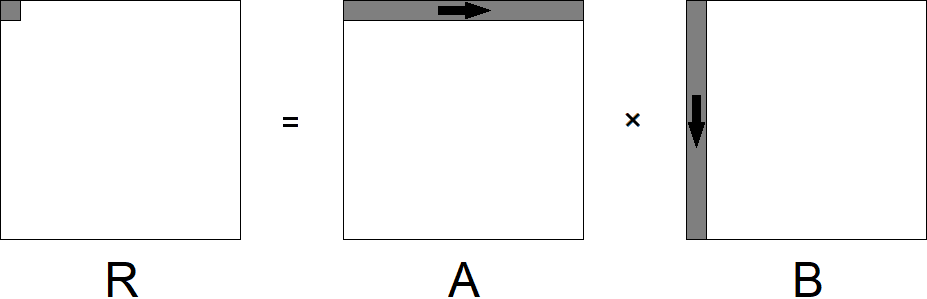
\includegraphics[width=\linewidth]{./images/3/lokIn.png}
	\caption{Zasoby wykorzystywane w pętli wewnętrznej}
	\label{fig:3inner}
\end{figure}

Powyższy rysunek przedstawia dokładnie, które dane są wykorzystywane do przetworzenia pętli w 6. linii kodu. Jak widać do wykonania jednej iteracji pętli wewnętrznej potrzebne jest odczytanie jednego wiersza macierzy $A$ i jednej kolumny macierzy $B$. Rezultatem tej pętli będzie odczytanie jednej wartości macierzy wynikowej $R$.

\begin{figure}[H]
	\centering
	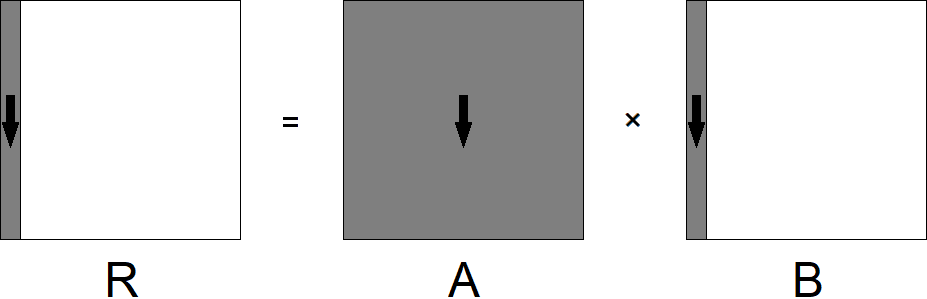
\includegraphics[width=\linewidth]{./images/3/lokMed.png}
	\caption{Zasoby wykorzystywane w pętli środkowej}
	\label{fig:3medium}
\end{figure}

Drugi rysunek ilustruje wykorzystanie danych do zrealizowania pętli w 5. wierszu. W tym przypadku potrzeba już wszystkich danych z macierzy $A$ i, tak jak w przypadku samej pętli wewnętrznej, jednej kolumny macierzy $B$. Otrzymujemy całą kolumnę macierzy wynikowej $R$. Wykonanie pętli zewnętrznej pozwoli na uzyskanie wartości wszystkich kolumn macierzy $R$ i będzie wymagało wszystkich danych z macierzy $A$ i $B$.

Dyrektywy OpenMP w 2. i 3. wierszu wykorzystano do uruchomienia kodu na wielu wątkach oraz podzielenia przetwarzania pętli między nimi. Kolejne iteracje pętli w 4. wierszu zostaną przydzielone równomiernie między wątki. Spowoduje to, że kolumny macierzy $B$ i macierzy wynikowej $R$ nie będą się powtarzały w kolejnych wątkach.

\subsubsection{Algorytm dla 5. wersji kodu}
\begin{lstlisting}[
caption={5. wersja kodu},
label=2. funkcja,
firstnumber=9]
template <int BLOCK_SIZE> __global__ void
matrixMul3(float *C, float *A, float *B, int wA, int wB ) {
    int bx = blockIdx.x;
    int by = blockIdx.y;
    
    int tx = threadIdx.x;
    int ty = threadIdx.y;
    
    int aBegin = wA * BLOCK_SIZE * by;
    int aEnd   = aBegin + wA - 1;
    int aStep  = BLOCK_SIZE;
    int bBegin = BLOCK_SIZE * bx;
    int bStep  = BLOCK_SIZE * wB;
    
    float Csub = 0;

    __shared__ float As[BLOCK_SIZE][BLOCK_SIZE];
    __shared__ float Bs[BLOCK_SIZE][BLOCK_SIZE];

    for (int a = aBegin, b = bBegin; 
    	 a <= aEnd;
    	 a += aStep, b += bStep) {
        As[ty][tx] = A[a + wA * ty + tx];
        Bs[ty][tx] = B[b + wB * ty + tx];
        
        __syncthreads();
        
#pragma unroll

        for (int k = 0; k < BLOCK_SIZE; ++k) {
            Csub += As[ty][k] * Bs[k][tx];
        }

        __syncthreads();
    }
    
    int c = wB * BLOCK_SIZE * by + BLOCK_SIZE * bx;
    C[c + wB * ty + tx] = Csub;    
}
\end{lstlisting}

Druga funkcja jest bardziej złożona. Wydaje się, że 3 wewnętrzne pętle działają podobnie do pętli w poprzedniej funkcji pracując tylko dla określonego fragmentu każdej z macierzy (wielkość tego obszaru jest określona w argumencie $r$). W rzeczywistości działanie tych 3 pętli odbiega trochę od tego, co obserwowaliśmy przy okazji analizy poprzedniej funkcji. Jest to spowodowane inną kolejnością odpowiadających pętli (w pierwszej funkcji kolejność jik, w drugiej ii,kk,jj).

\begin{figure}[H]
	\centering
	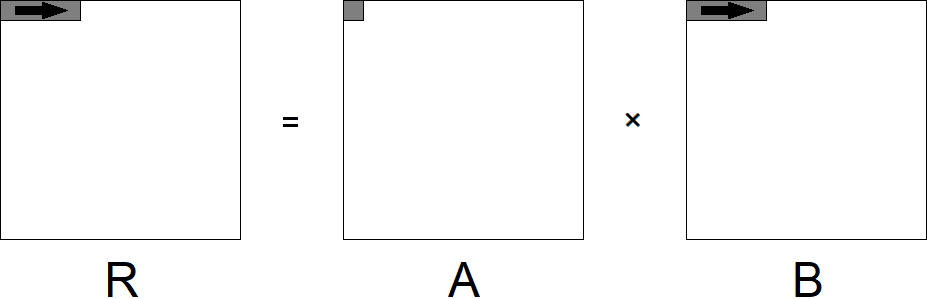
\includegraphics[width=\linewidth]{./images/6/lokIn1.png}
	\caption{Zasoby wykorzystywane w pętli w 17. wierszu}
	\label{fig:6inner1}
\end{figure}

\begin{figure}[H]
	\centering
	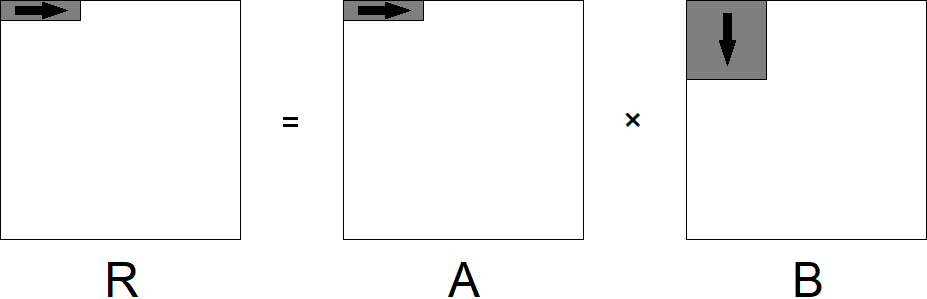
\includegraphics[width=\linewidth]{./images/6/lokIn2.png}
	\caption{Zasoby wykorzystywane w pętli w 16. wierszu}
	\label{fig:6inner2}
\end{figure}

\begin{figure}[H]
	\centering
	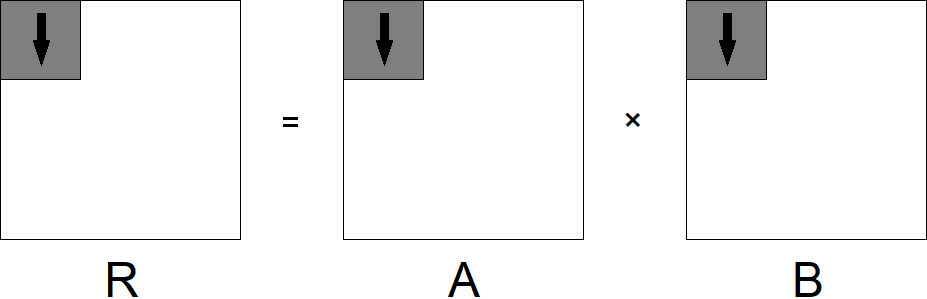
\includegraphics[width=\linewidth]{./images/6/lokIn3.png}
	\caption{Zasoby wykorzystywane w pętli w 15. wierszu}
	\label{fig:6inner3}
\end{figure}

Trzeci rysunek pokazuje, które dane są brane pod uwagę podczas wykonywania danej pętli. Uzyskujemy wiersz fragmentu macierzy $R$, którego wartości są iloczynem jednego elementu macierzy $A$ i wartości któregoś z wierszy odpowiadającego fragmentu w macierzy $B$. Uzyskane wartości nie są jednak wartościami ostatecznej macierzy wynikowej. Czwarty rysunek pokazuje, że kolejna pętla w dalszym ciągu oblicza wartości dla tych samych komórek macierzy $R$ poprzez sumowanie iloczynów elementów leżących w jednym wierszu fragmentu macierzy $A$ i wszystkich komórek fragmentu macierzy $B$. Najbardziej zewnętrzna pętla uzyskuje już wartości dla całego fragmentu i, jak pokazuje piąty rysunek, potrzeba do tego wszystkich wartości w odpowiadających fragmentach macierzy $A$ i $B$. Otrzymane wartości również nie są wartościami ostatecznymi. Dopiero kolejna pętla sprawi, że otrzymamy wartości fragmentu macierzy wynikowej $R$.

\begin{figure}[H]
	\centering
	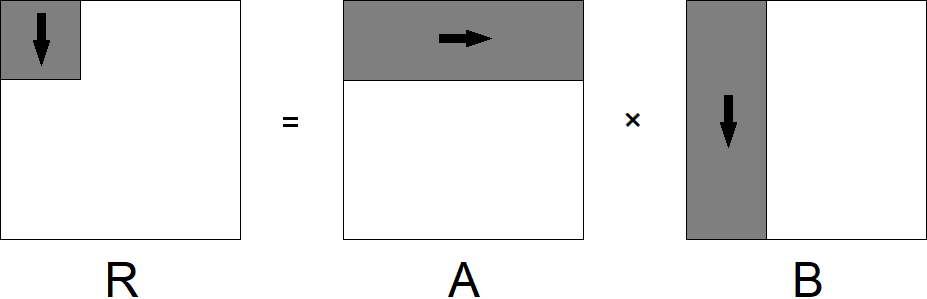
\includegraphics[width=\linewidth]{./images/6/lokMed.png}
	\caption{Zasoby wykorzystywane w pętli w 14. wierszu}
	\label{fig:6medium}
\end{figure}

Jak widać w powyższym rysunku, ta pętla wykorzystuje już całe wiersze i kolumny macierzy $A$ i $B$. W tej pętli odbywa się zsumowanie wartości odpowiadających elementów różnych fragmentów funkcji, które są pokrywane przez te wiersze i kolumny. W efekcie otrzymamy wartości, które złożą się w ostatecznym rozrachunku na całą macierz wynikową R.

\begin{figure}[H]
	\centering
	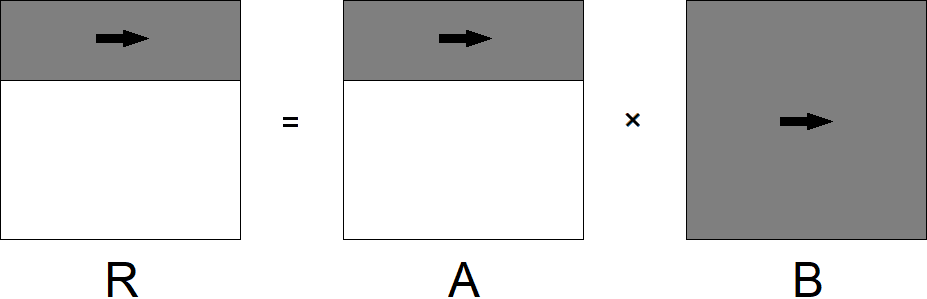
\includegraphics[width=\linewidth]{./images/6/lokOut1.png}
	\caption{Zasoby wykorzystywane w pętli w 13. wierszu}
	\label{fig:6outer1}
\end{figure}

Ostatnie dwie pętle odpowiadają za wybór fragmentu, którego elementy zostaną w następnych pętlach obliczone. Powyższy rysunek przedstawia wykorzystanie danych w tej wewnętrznej. Jak widać potrzebuje ona $r$ wierszy i wszystkich elementów macierzy $B$. Zewnętrzna będzie już potrzebowała całych macierzy $A$ i $B$. Złożoność tego rozwiązania wynosi $O((\frac{n}{r})^3*r^3)=O(n^3)$.

Dyrektywy OpenMP działają podobnie jak w pierwszej funkcji. Tutaj pomiędzy wątki równomiernie zostają rozdzielone kolejne iteracje pętli w 13. wierszu.

\subsection{Analiza efektywności}
\subsubsection{Podział pracy na wątki}

W pierwszej funkcji wątek dokonuje obliczeń dla pojedynczej kolumny macierzy wynikowej $R$ co odpowiada sytuacji na rysunku 2. Wykorzystuje do tego jedną kolumnę macierzy $B$ i całą macierz~$A$. Dla drugiej funkcji zrównoleglenie odbywa się dla pętli w 13. wierszu, a więc wątki dokonują obliczeń dla mniejszego fragmentu macierzy wynikowej $R$ o rozmiarze $r x r$, gdzie $r$ jest argumentem funkcji. Dane wykorzystywane przez jeden wątek dla tej funkcji przedstawia rysunek 6.

\subsubsection{False sharing}

W pierwszej funkcji do wyliczenia fragmentu macierzy $R$, za który dany wątek jest odpowiedzialny, potrzebuje on dostępu do kolumny macierzy $B$, której żaden inny wątek nie będzie potrzebował. Niestety nie dotyczy to dostępu do macierzy $A$. Tutaj każdy wiersz będzie musiał być udostępniony do wszystkich wątków, zatem może dojść do sytuacji, kiedy wątki uzyskają równoczesny dostęp do danych znajdujących się blisko siebie w pamięci podręcznej i do ich unieważnienia przez inne wątki. Prowadzi to do konieczności ponownego pobrania danych co finalnie spowolni obliczenia.

W drugiej funkcji false sharing również może zajść. Wątki będą zmuszone do obliczania tych samych fragmentów macierzy, co inne wątki, aby je zsumować i otrzymać ostateczne wartości fragmentu macierzy $R$, za który dany wątek jest odpowiedzialny. W tej sytuacji jednak wątki będą korzystać w danej chwili z krótszych wierszy o długości $r$, dzięki czemu unieważniane będą znacznie mniejsze fragmenty pamięci podręcznej. W porównaniu z pierwszą funkcją, w której może dojść do unieważniania całych wierszy, w tym przypadku nie powinno to wpłynąć w tak dużym stopniu na czas. 

\subsubsection{Analiza lokalności dostępu do danych}

Rozróżniamy dwa rodzaje lokalności -- czasową i przestrzenną. Pierwsza oznacza wielokrotne odwoływanie się wątków do tych samych danych przetrzymywanych w pamięci podręcznej. Do jej wystąpienia wymagane jest odpowiednio duży rozmiar pamięci podręcznej, która musi być większa od rozmiaru pamięci potrzebnej do wykonania danej operacji i będzie tak dla wszystkich analizowanych poniżej przypadków. Lokalność przestrzenna polega na dostępie do danych występujących jeden po drugim w pobranej linii pamięci czyli w jednym wierszu macierzy.

\paragraph{Lokalność dla pierwszej funkcji}

\begin{itemize}

\item Dla pętli wewnętrznej

Zużycie danych przedstawia rysunek 1. Dla macierzy $R$ mamy lokalność odwołań, gdyż jeden wątek w każdej iteracji tej pętli odwołuje się do tej samej komórki macierzy $R$. Dla macierzy $A$ uzyskamy natomiast lokalność przestrzenną.

\item Dla pętli środkowej

Wykorzystanie danych przez jeden wątek w tej sytuacji przedstawia rysunek 2. 

Wątek w danej iteracji tej pętli jest odpowiedzialny za jedną kolumnę macierzy $R$. Taka sytuacja jest przedstawiona na drugim rysunku. Potrzebna jest cała macierz $A$ i jedna kolumna macierzy $B$. Do otrzymania jednej komórki dla wynikowej kolumny będzie potrzebny jeden wiersz macierzy $A$, wykorzystujemy więc całe linie pamięci. Mamy zatem do czynienia z lokalnością przestrzenną. Lokalność czasowa zależy od dostępnej pamięci podręcznej.

\end{itemize}

\paragraph{Lokalność dla drugiej funkcji}

\begin{itemize}

\item Dla pierwszej pętli wewnętrznej - wiersz 17.

Zużycie danych przedstawia rysunek 3. Ze względu na niewielką ilość przetwarzanych komórek przy odpowiednio małym $r$ wystąpi tutaj lokalność czasowa. Dla macierzy $R$ i $B$ mamy lokalność przestrzenną, natomiast dla macierzy $A$ będziemy mieli lokalność odwołań, bo odwołujemy się cały czas do jednej komórki.

\item Dla drugiej pętli wewnętrznej - wiersz 16.

Sytuacja bardzo zbliżona do tej powyższej. Przedstawia ją kolejny rysunek nr 4. Lokalność przestrzenna wystąpi tutaj dla wszystkich macierzy, lokalność czasowa jest też bardzo prawdopodobna i zależy od $r$.

\item Dla trzeciej pętli wewnętrznej - wiersz 15.

Wykorzystanie danych przedstawione na rysunku 5. Tak samo jak w powyższych przypadkach, mamy tutaj do czynienia z lokalnością przestrzenną i czasową, jeśli oczywiście wartość $r$ jest odpowiednio mała.

\end{itemize}

Dla bardziej zewnętrznych pętli lokalność, szczególnie przestrzenna może być trudna do uzyskania, jednak samo występowanie lokalności dla 3 wewnętrznych pętli może zapewnić dużą lokalność dostępu do danych dla całego algorytmu i może skutkować krótszym przetwarzaniem danych dzięki większej skuteczności trafień danych w pamięci podręcznej. Same wielkości macierzy nie powinny mieć tu dużego wpływu na uzyskanie lokalności. Rolę tutaj odgrywa wielkość $r$, która musi być na tyle mała aby pamięć podręczna zmieściła 3 fragmenty macierzy $R$, $A$ i $B$ o rozmiarach $r$ x $r$.

Jeśli wielkość rozpatrywanego fragmentu macierzy w drugiej funkcji wynosi $r$, a wielkość pamięci podręcznej cache $M$, to zależność między tymi wartościami przedstawia się następująco:
\[ 3*r*r*6 \leq M \Longleftrightarrow r \leq \sqrt{M/3}/6\]
Dzielenie przez 6 wynika z ilości jednocześnie uruchomionych wątków. Aby zadbać o jak najszybsze przetwarzanie powinniśmy zadbać, aby stosowane zmienne nie przekroczyły wielkości pamięci L3, która ma wielkość 8 MB. Przekroczenie pojemności tej pamięci powoduje znaczne spowolnienie działania algorytmu. Zmiennych typu float (rozmiar 4B) na których przeprowadzane są obliczenia, możemy przechować: 
\[ M = 8MB/4B = 2 * 1024 * 1024 = 2097152 \]
Wartość $r$ wynosi zatem:
\[ r \leq \sqrt{2097152 / 3}/6 \]
\[ r \leq \sqrt{699050,67}/6 \]
\[ r \leq 836,09/6 \]
\[ r \leq 139,35 \]
Największa optymalna wartość $r$ dla rozważanej pamięci cache, która pozwoli na zachowanie dużej lokalności drugiego algorytmu wynosi wobec tego $139$.

\section{Analiza przetwarzania}
\subsection{Przebieg}

Dla danego problemu istnieje instancja graniczna, ze względu na ograniczoną pojemność pamięci podręcznej L3. Tak jak już rozważaliśmy przy analizie lokalności, dla pamięci L3 możemy przechowywać $2097152$ zmiennych typu float. Pamięć L3 jest współdzielona przez wszystkie rdzenie procesora, więc dane które nie mieszczą się w L3, muszą zostać przeniesione do pamięci RAM, co powoduje zwiększenie czasu przetwarzania.

W wersji algorytmu 3 pętlowej, każdy wątek musi załadować do pamięci kolumnę macierzy wynikowej $R$, całą macierz $A$ oraz kolumnę macierzy $B$.
Należy zatem posłużyć się wzorem:
\[ n_R + n_A^2 + n_B < 2097152 \]
Wynikiem jest:
\[ n_R = n_A = n_B = 1447\]
Eksperyment zostanie przeprowadzony na trzech rozmiarach instancji: 1400, 1500 oraz 1600.


\subsection{Wyniki}
\subsubsection{Instruction per Cycle}
Instruction per Cycle, czyli w skrócie IPC, jest to stosunek wykonanych istrukcji i liczby cykli zegara, im większa jest to wartość, tym więcej wykonujemy instrukcji na cykl, a więc wykorzystanie procesora jest lepsze.

\begin{figure}[H]
	\centering
	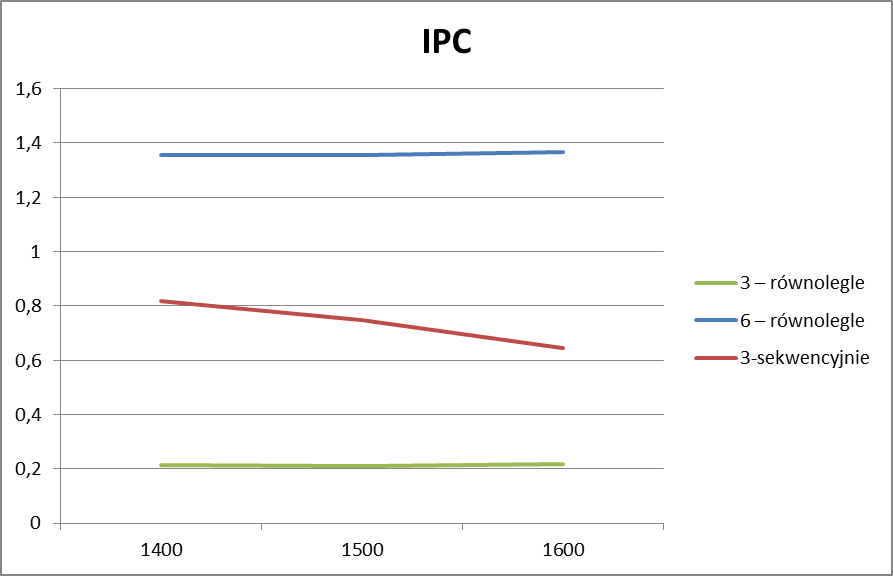
\includegraphics[width=\linewidth]{./images/wykresy/IPC.png}
	\caption{Instruction per Cycle}
	\label{fig:wykres1}
\end{figure}

\subsubsection{Data cache miss ratio}
Data cache miss ratio jest to stosunek nietrafień do pamięci podręcznej i wszystkich dostępów zrealizowanych. Im mniejszy jest ten wynik, tym rzadziej trzeba odwoływać się dalej, niż do pamięci podręcznej. 

\begin{figure}[H]
	\centering
	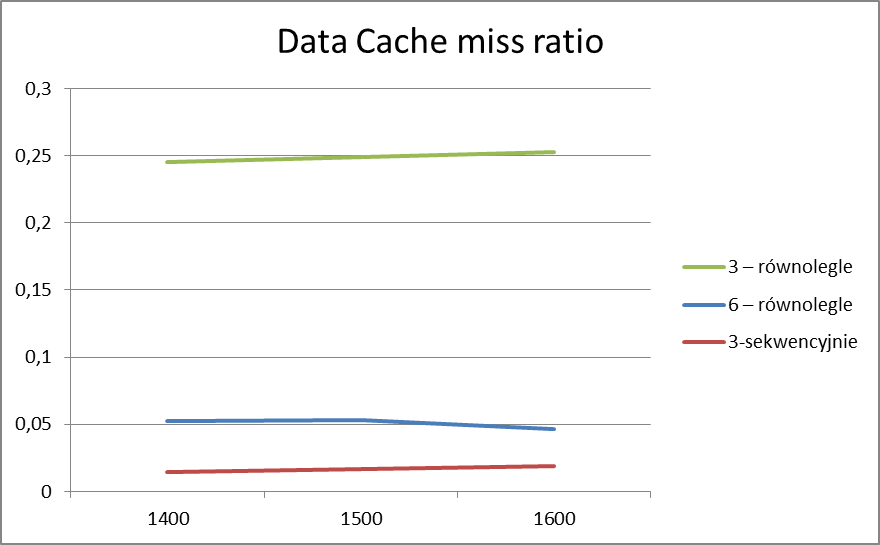
\includegraphics[width=\linewidth]{./images/wykresy/miss_ratio.png}
	\caption{Data cache miss ratio}
	\label{fig:wykres2}
\end{figure}

\subsubsection{Data cache miss rate}
Data cache miss rate jest stosunkiem nietrafień do pamięci podręcznej i wykonanych instrukcji. Im większa jest ta wartość, tym wolniej realizowane jest przetwarzanie.  

\begin{figure}[H]
	\centering
	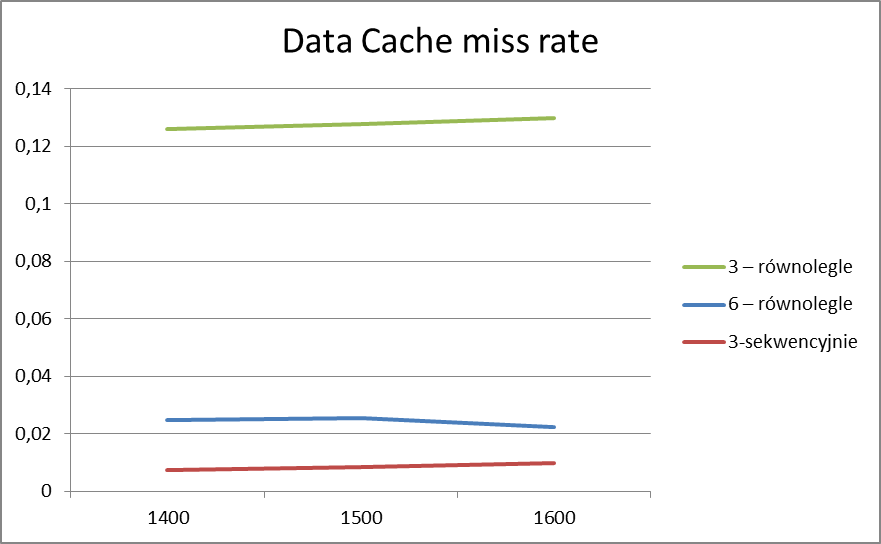
\includegraphics[width=\linewidth]{./images/wykresy/miss_rate.png}
	\caption{Data Cache miss rate}
	\label{fig:wykres3}
\end{figure}

\subsection{Analiza przyspieszenia}

Algorytmy równoległe, zarówno trójpętlowe, jak i  sześciopętlowe, zostały porównane pod względem czasu przetwarzania z algorytmem sekwencyjnym. Wykres przedstawia iloraz czasu przetwarzania najlepszej znanej metody sekwencyjnej i czasu obliczeń równoległych.

\begin{figure}[H]
	\centering
	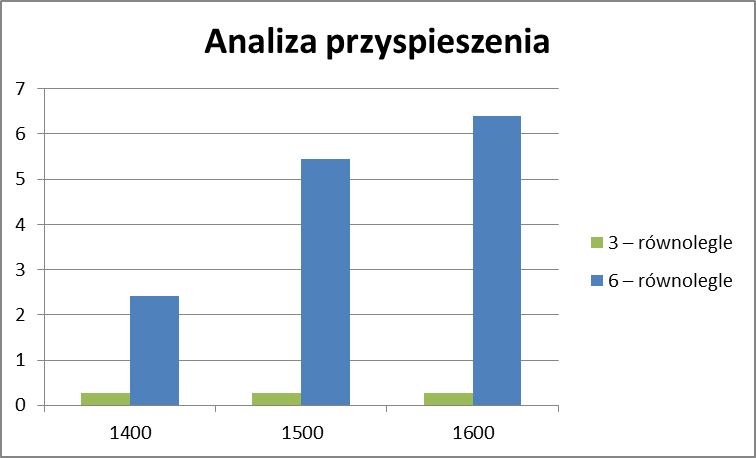
\includegraphics[width=\linewidth]{./images/wykresy/analiza_przyspieszenia.png}
	\caption{Analiza przyspieszenia}
	\label{fig:wykres4}
\end{figure}

Wykres pokazuje, że realizacja równoległa za pomocą metody 3 pętlowej wypada zdecydowanie gorzej niż metoda sekwencyjna. Kolejność JIK mnożenia macierzy wypada wyjątkowo słabo. Spowodowane to jest słabą lokalnością przestrzenną danych, iteracje używają całych kolumn, które wymagają sprowadzania całych wierszy z pamięci. Z tego powodu często pojawiają się nietrafienia do pamięci podręcznej z powodu jej ograniczonej pojemności. Przetwarzanie za pomocą kolumn sprawia, że pojawia się problem false sharingu, który dodatkowo niekorzystnie wpływa na czas przetwarzania.

Wersja sześciopętlowa ijk, iikkjj, osiąga nawet 6 krotnie przyspieszenie względem wersji sekwencyjnej. Im większa instancja tym większa korzyść wynika z użycia algorytmu dzielącego macierz na podmacierze. Mniej danych trzeba jednocześnie sprowadzać do pamięci współdzielonej, więc nie następuje przepełnienie jej. Z tego powodu nie trzeba odwoływać się do wolniejszych pamięci i całe przetwarzanie realizowane jest szybciej. 

\section{Wnioski}
Nieodpowiedni dobór algorytmu równoległego do zadania nie tylko powoduje nie uzyskanie przyspieszenia przetwarzania, ale także może spowodować znaczne spowolnienie względem wersji sekwencyjnej. Przed zastosowaniem algorytmu równoległego, należy przeprowadzić dogłębną analizę sposobu przetwarzania danych przez algorytm, aby wybrać jego optymalną implementację.
\end{document}
